\section{Bistatic Clutter Impacts}

As previously discussed, the Signal to Clutter Ratio (SCR) is a valuable metric that determines the observability of a target against the background. Clutter is very well understood for monostatic geometries but still an active area of research for bistatic geometries.

\subsection {Bistatic Clutter Estimation}
Because the RCS varies by target and both signal and clutter are captured under the same conditions, we can focus on the Clutter Cross Section (CCS) to get a relative sense of how background clutter relates to bistatic RADAR.

We can use Long's model \cite{griffiths_bistatic_clutter} to determine the cross range clutter backscatter term, $\sigma_{Mx}^0$. This term is dependent on wind speed, $v_w$ and wind direction, $\phi_w$.
\begin{equation}
\sigma_{Mx}^0 = 29.8\log\left(0.5144 v_w\right) + 6\cos\left(\phi_w \right) -84.7
\label{bc_eq:1}
\end{equation}
\renewcommand{\baselinestretch}{2} \small\normalsize

We can then use $\sigma_{Mx}^0$ to find the bistatic clutter backscatter strength, $\sigma_{B}^0$
\begin{equation}
\sigma_B^0 = 10\log\left[\sqrt{\sigma_M^0(\theta_1,0)\sigma_M^0(\theta_2,\phi)} |\cos(\phi)|^m  + k\sqrt{\sigma_{Mx}^0(\theta_1,0)\sigma_{Mx}^0(\theta_2,\phi)}|\sin(\phi)|^n \right]
\label{bc_eq:2}
\end{equation}
\renewcommand{\baselinestretch}{2} \small\normalsize

Here, $\theta_1$ is the grazing angle relative to the receiver, $\theta_2$ is the grazing angle relative to the transmitter, $phi$ is the azimuth angle between the receiver and transmitter, $\sigma_M^0$ is the monostatic clutter backscatter strength. In addition, $k$, $m$, and $n$ are model "fudge-factors" that must all be positive. The $\cos(\phi)$ term captures the downrange component and the $\sin(\phi)$ term captures the cross range component.

The NRL model for downrange clutter backscatter averages the backscatter responses for all wind directions and therefore effects of wind direction are not described in the model. Like the NRL model, Long's model for crossrange clutter backscatter is based on empirical data relating sea clutter to polarization and wind direction, however Long's model averages over a range of sea states rather than resolving it in the model. As a result, the inherent variance in the combined model is handled by fudge factors to adapt to environments of a given sea state and wind direction.

An example image that shows a bistatic clutter map with the propagation factors superimposed is given in Figure \ref{bc_fig:1}. 

\begin{figure}[H]
  \begin{center}
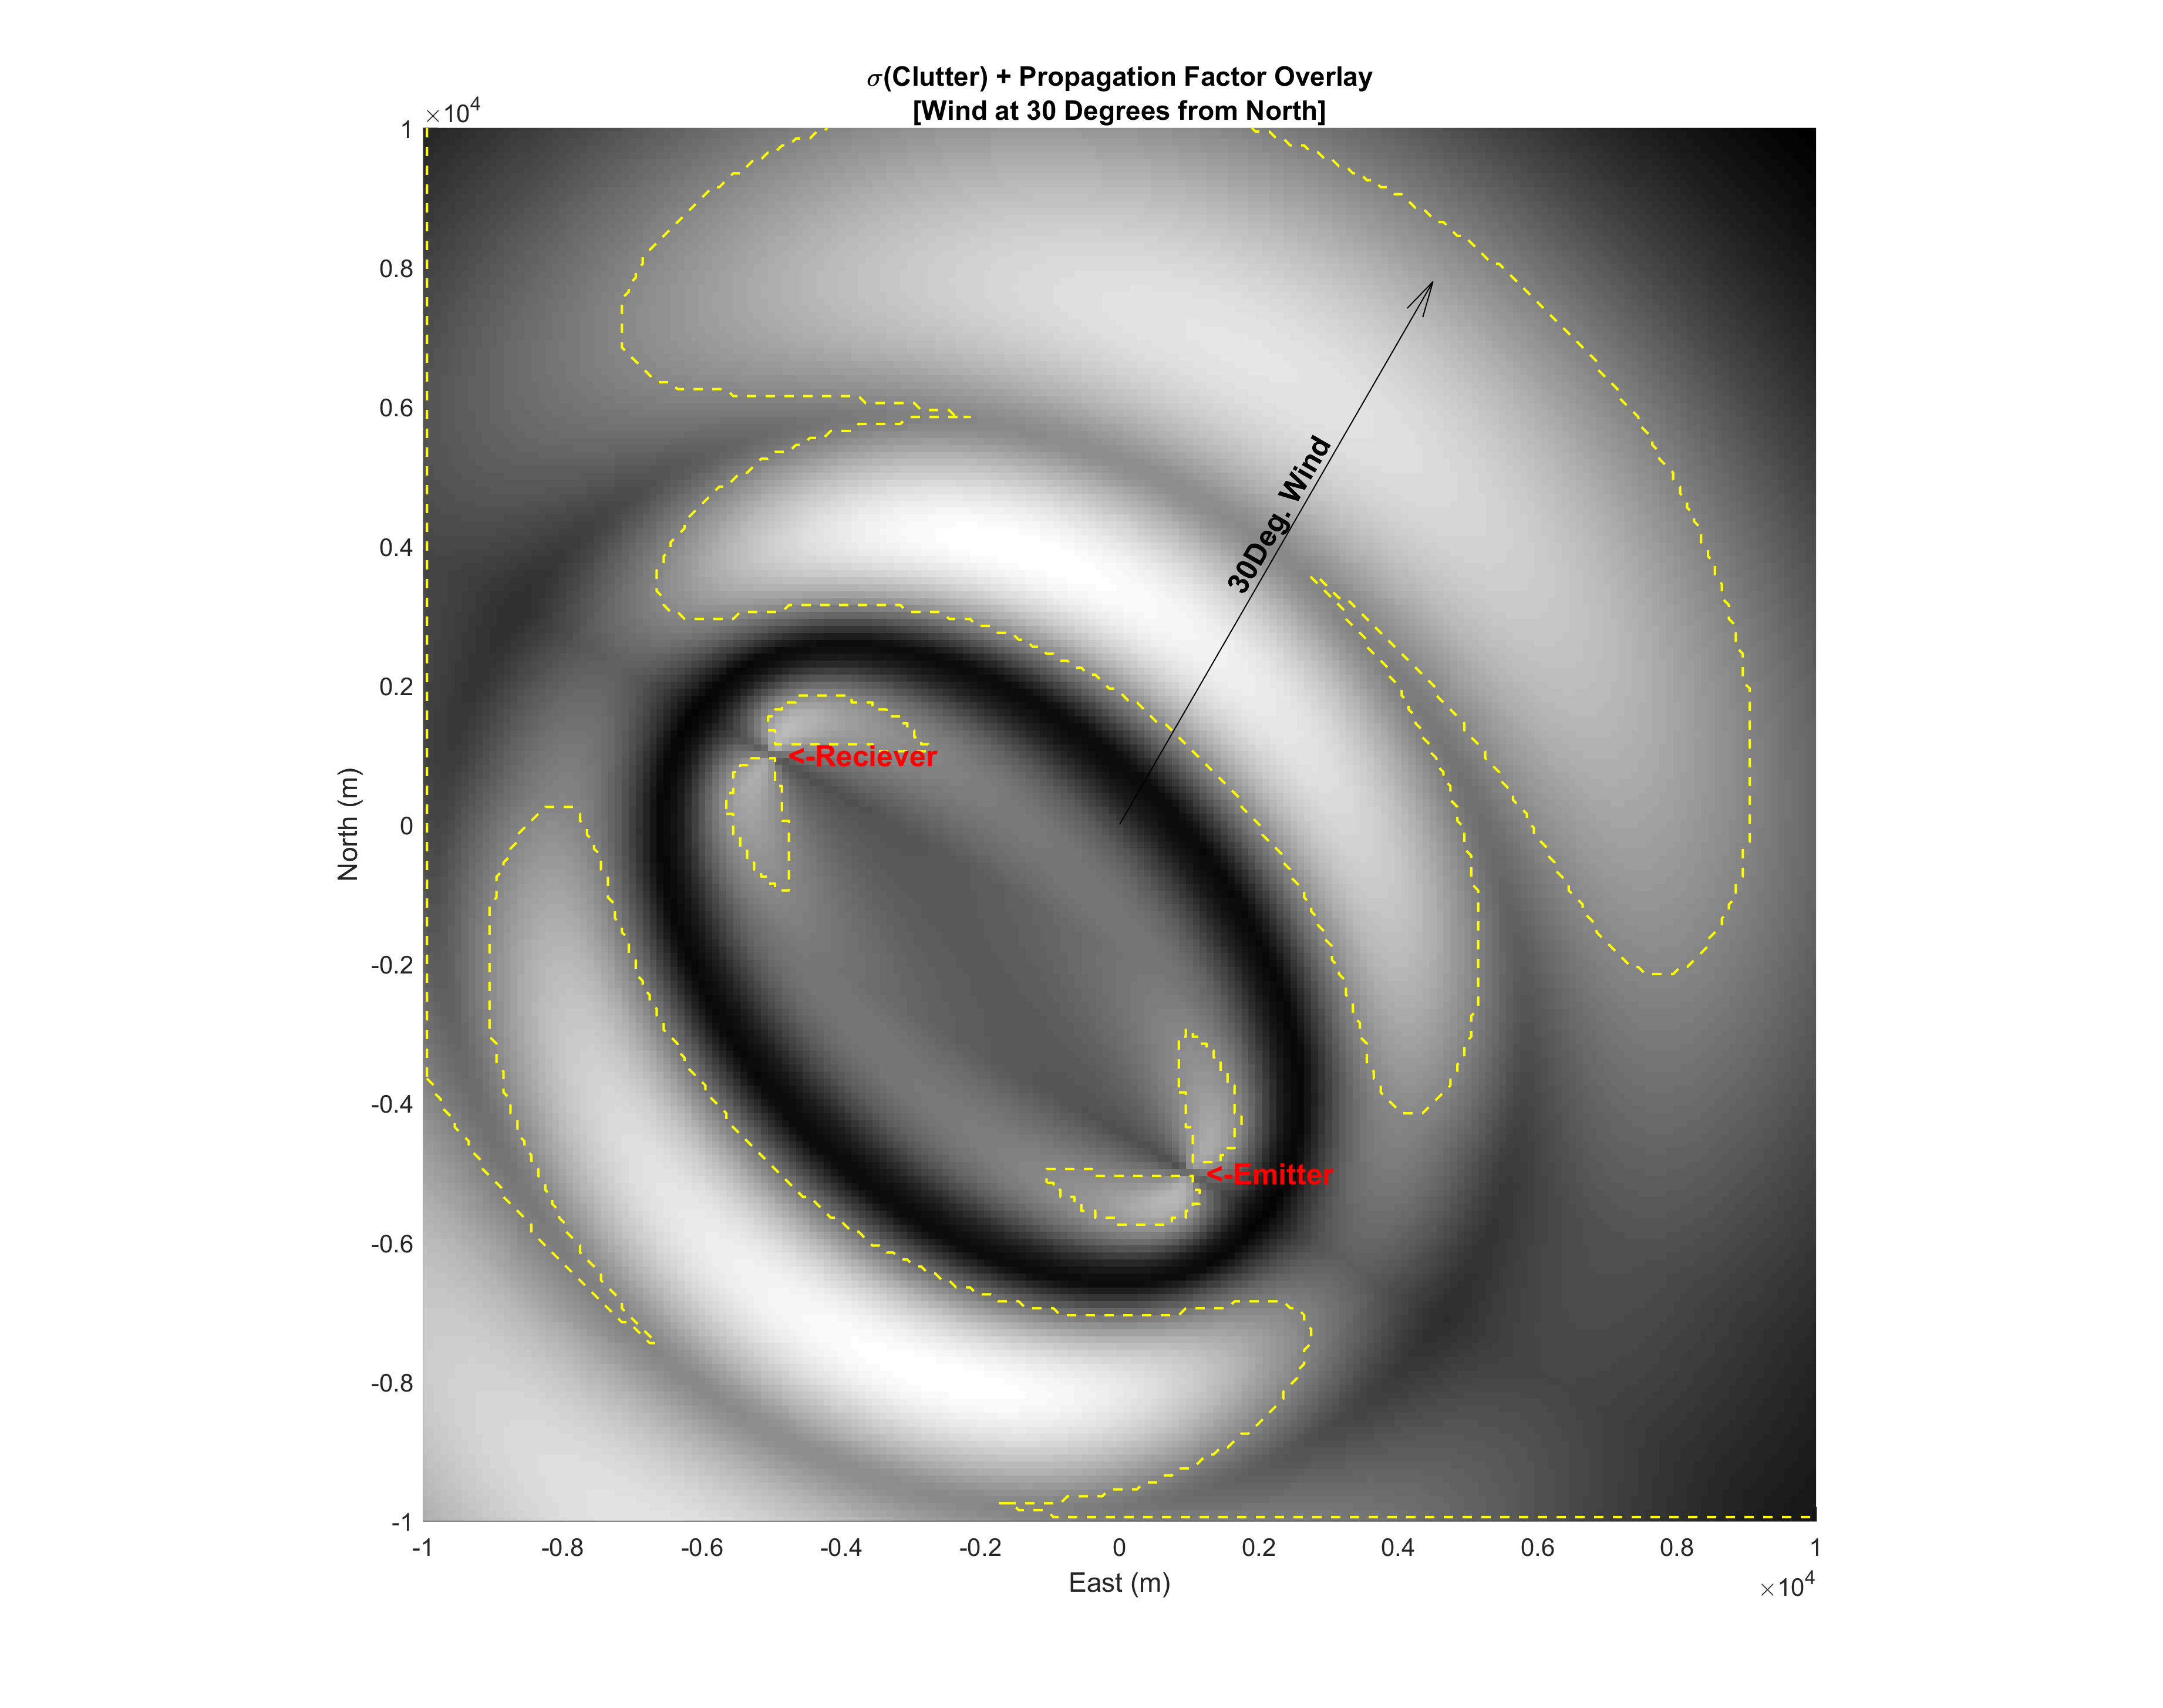
\includegraphics[width=5in]{../media/analysis/FpCCSOverlay.png}
  \end{center}
  \renewcommand{\baselinestretch}{1} \small\normalsize
  \begin{quote}
    \caption[Clutter and $F_p$ Overlay]{Clutter and $F_p$ Overlay\label{bc_fig:1}}
  \end{quote}
\end{figure}
\renewcommand{\baselinestretch}{2} \small\normalsize